\chapter{Discussion des résultats}


%Analyse globale des résultats, discussion sur les résultats 
%Données manquantes

%Exemple: on sait que la fermentation du grain dans sa pulpe impacte sur la chimie de la graine et peut rendre le café plus ou moins acide -> pas de données sur la fermentation (temps, méthode etc) idem pour le séchage, le stockage, la récolte etc


% L'objectif aurait été de définir des gouts (tastewheel ) - pas de données

% Revenir sur les données 

% todo -> améliorer les modèles, changer les index (RMSE, RSquared etc) - nécessite théorie

% Portes qui s'ouvrent 

%TODO - Relire et relire, revenir surle rapport et relire, penser au résumé etc

Les différentes analyses réalisées, tant au niveau de l'apprentissage supervisé que non-supervisé n'ont pas permis de créer un modèle fiable de description ou de prédiction de la qualité du café. Cependant, certains résultats peuvent être mis en avant et certaines critiques peuvent être faites sur les données et les méthodes utilisées. \\

%Relation avec la pluie
\paragraph{Résultats exploitables} Concernant les résultats exploitables, une relation a été observée entre la quantité de pluie durant l'année et le nombre de défauts physiques du grain. Plus il y a de pluie, plus il y a de grains ayant des défauts et plus il y a de cafés ayant la note zéro (voir figure \ref{ThirdSOMASNM}). Rappelons que les grains défectueux sont éliminés par un processus industriel permettant l'élimination des grains ayant une couleur ou une densité anormale. Cependant, certains défauts, comme la présence de trous dûs aux parasites (Broca, ou Broca de punto), sont plus difficilement détectables et peuvent amener un goût désagréable au café. Un seul grain peut modifier le goût d'une tasse ! On remarque aussi que l'année 2011 a beaucoup moins de cafés dont la note dépasse les 80 (voir figure \ref{fig:pointtotauxetc}), score minimal pour avoir ma mention \textit{Specialty Coffee}. Il est donc raisonnable de penser que les fortes quantités de pluie, nuisent à la qualité du café et que plus il pleut, moins il y a de chance d'avoir de très bon cafés.  \\



% Manque de données
\paragraph{Données disponibles} Certain points concernant la qualité des données reçues sont à mettre en avant. Premièrement, les données de qualités de sols ne contenant que le pH, le taux de matières organiques et la texture, toute les relations chimiques éventuelles entre les minéraux du sol et les arômes n'ont pas pu être explorées. La composition chimique du sol n'est pas la seule à avoir une influence possible sur la qualité et les saveurs du café. Les différents traitement du café une fois récoltés, comme la fermentation ou le séchage, peuvent avoir une grande influence mais malheureusement aucune donnée n'a été fournie à ce sujet non plus. \\

\noindent Deuxièmement, les données de dégustation contenaient parfois, de manière difforme, des notes sur les arômes ou saveur du café. Ces données peuvent être décrite comme sur la figure \ref{fig:coffeeflavorwheel} et pourraient permettre de décrire d'une manière plus sensorielle le goût du café et et ainsi faire un éventuel lien avec les composants chimiques du sol et les pratiques culturales ou même le climat. Malheureusement le manque de données en nombre d'une part et d'uniformité d'autre part n'ont pas permis d'intégrer ces informations au set de données et donc d'en analyser les éventuelles corrélations.\\

\begin{figure}[h]
	\centering
	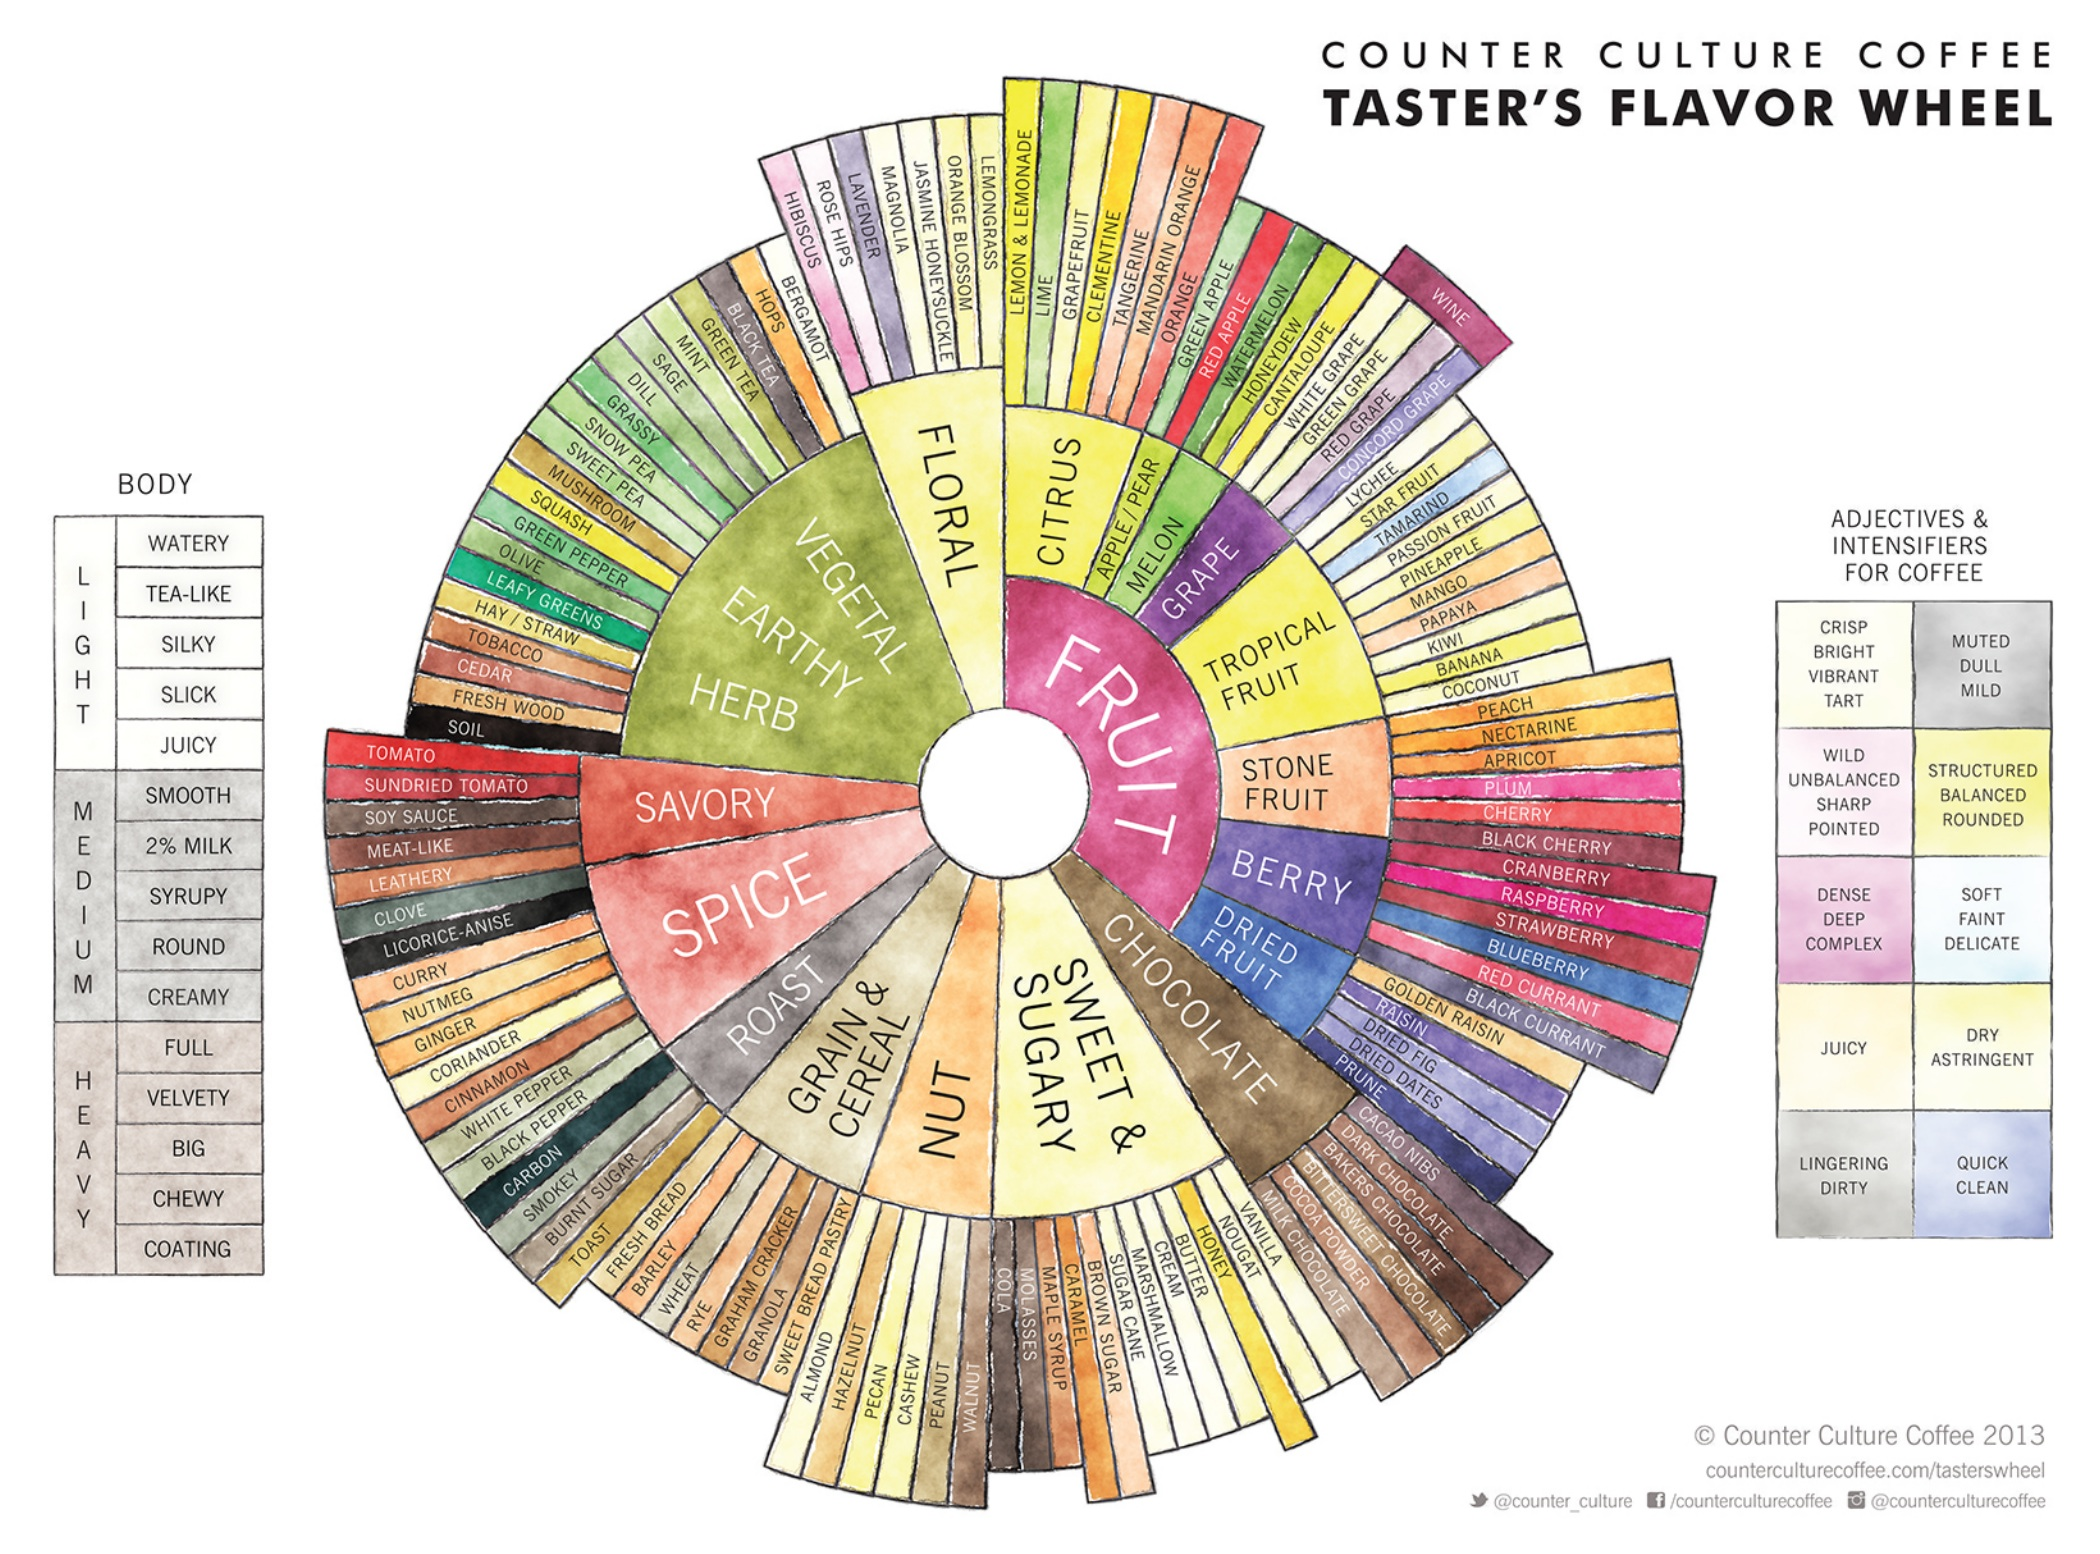
\includegraphics[width=1\linewidth]{img/coffee_flavor_wheel}
	\caption{Roue des parfums du café}
	\label{fig:coffeeflavorwheel}
\end{figure}



%Customisation des méthodes, essais avec d'autres méthodes, traitement des variables catégorielles

%parler des données d'Eric sur la plante du café, de la taille etc



\noindent Il serait intéressant de prélever d'autres données, directement au niveau des fermes. Beaucoup de facteurs influence la croissance d'une plante et la maturation de ses fruits en particulier les facteurs influençant la photosynthèse. Si une plante est particulièrement exposée à l'est, et donc au soleil du matin, la photosynthèse sera plus efficace car l'humidité ambiante est plus élevée. Par contre, si la plante grandit sur un terrain ombragé, donc entourée d'autres plantes, l'humidité sera aussi plus élevée mais la plante devra fabriquer plus de feuilles pour capter plus de lumière et aura donc moins d'énergie à mettre dans les fruits. L'altitude peut aussi avoir une influence importante sur les conditions. Sur la luminosité, en particulier par rapport à la couverture nuageuse mais aussi sur la température. Dans les lieux plus froids, la plante fonctionne plus lentement et les fruits ont besoin de plus de temps pour murir, ce qui laisse plus de temps aux arômes pour se développer et produit de manière générale des cafés de qualités.  \\



% si on veut prédire la qualité du café, il faut des données précises. Il peut pleuvoir des trombes sur une ferme, et 100m plus loin rien. 



%Résultat
\noindent Durant le projet, une réunion a été organisée avec Felipe Rincón, coordonnateur de gestion au comité départemental des caféiculteurs de Risaralda, qui est à l'origine des données sur le café que nous avons reçues. La possibilité m'a été donnée de poser des questions entre autre sur le processus de récolte et de centralisation des données, processus jusqu'alors inexistant. M. Rincón m'a alors confié que les différentes demandes effectuées pour ce travail ainsi que le résultat final de l'agglomération des données disponibles, l'ont poussé à commencer un processus de normalisation de la récolte des données. Il est donc envisageable de pouvoir retenter une étude de ce type lorsque les données existantes auront éventuellement complétées et lorsque de nouvelles données, plus complètes et possédant moins de défauts, auront été générées. Parmi les défauts importants signalés à M. Rincón, on notera qu'aucune date de récolte n'a été fournie. Seul les dates de dégustation étaient disponibles et les périodes de croissance de la plante ont dû être estimées. \\


\paragraph{Méthodes utilisées} Il est aussi important de mentionner les méthodes utilisées. Random Forest, PLS, ou le clustering, peuvent être paramétrées de beaucoup de manières différentes et leur efficacité peut être testée et améliorée. Dans le cadre de ce projet, avec le peu d'heures à disposition, ces méthodes ont été utilisées de manière exploratoire afin d'avoir une première impression sur les possibilités de modélisation. D'un même point de vue, d'autres méthodes auraient pu être explorées en jouant sur les particularités de chacune d'entre-elles par rapport aux types de données en notre possession. Pour améliorer cette partie, un bagage théorique supplémentaire en statistique serait nécessaire afin de mieux cerner les subtilités des méthodes de modélisation.  \\

\noindent 


 













